\section{Криволинейные интегралы}
\subsection{Интегралы I рода}
Физический смысл ~---~ это масса кривой с заданной плотностью.
\begin{definition}
    Будем говорить, что $f: [a, b] \rightarrow \R^n$ кусочно непрерывно-дифференцируема (кусочно 1-гладкая), если $f \in C([a, b], \R^n)$ и существует некоторое конечное разбиение \[T = \{t_i\}_{i = 0}^N, a = t_0 < t_1 < \ldots < t_N = b\] для которого верно следующее: \[\forall i \in \overline{0, N - 1} \hookrightarrow f|_{[t_{i}, t_{i + 1}]} \in C^1([t_i, t_{i + 1}], \R^n)\]
    А в самих точках существую односторонние производные.
\end{definition}
\begin{definition}
    Пусть $\Gamma = \{r(t) \mid t \in [a, b]\}$~---~кривая в $\R^n$, параметризованная кусочно 1-гладкой функцией $r$. Пусть $f \in C(\Gamma, \R)$. Тогда будем называть \textit{криволинейным интегралом I-го рода} $f$ по $\Gamma$:
    \[\int\limits_\Gamma f(r)ds := \int\limits_a^b f(r(t))\|r'(t)\|dt\]
\end{definition}
\begin{note}
    То что стоит слева это обозначение, а то что справа это расшифровка
\end{note}
\begin{lemma}
    Криволинейный интеграл I рода не зависит от выбора допустимой параметризации (сохраняющей ориентацию).
\end{lemma}
\begin{proof}
    Пусть $r(t) = \rho(\tau(t)) $~---~кусочно гладкая и $\Gamma = \{\rho(\tau) \mid \tau \in [\alpha, \beta]\}$, а $\tau(t)$~---~строго возрастающая гладкая функция, переводящая $[a, b]$ в $[\alpha, \beta]$. Тогда \[\int\limits_\alpha^\beta f(\rho(\tau))\|\rho'(\tau)\|d\tau = \int\limits_a^b f(\rho(\tau(t)))\|\rho'(\tau(t))\|\tau'(t)dt = \int\limits_a^b f(r(t))\|r'(t)\|dt\]
    (Это просто замена переменной в Риммановском интеграле. Поскольку $\tau(t)$~---~возрастающая, то $\tau' > 0$, и мы можем занести её под норму)
\end{proof}
\begin{lemma}
    Криволинейный интеграл I рода не изменяется при изменении ориентации.
\end{lemma}
\begin{proof}
    Пусть $r(t)$~---~допустимая параметризация кривой $\Gamma, t \in [a, b]$. Зададим $\rho(t) = r(-t), t \in [-b, -a]$. Тогда \[\int\limits_a^b f(r(t))\|r'(t)\|dt = -\int\limits_{-a}^{-b}f(r(-t)) \|r'(-t)\|d(-t) = \int\limits_{-b}^{-a}f(\rho(t))\|\rho'(t)\|dt\]
\end{proof}
\subsection{Интегралы II рода}
Физический смысл ~---~ это работа силы вдоль траектории.

\begin{definition}
    Пусть $\Gamma = \{\overline{r}(t) \mid t \in [a, b]\} \subset \R^n$~---~ориентированная кривая, параметризованная кусочно-гладкой $r: [a, b] \rightarrow \R^n$. Пусть $
    \overline{F} \in C(\Gamma, \R^n)$. Тогда \textit{криволинейным интегралом II-го рода} $f$ по $\Gamma$ будем называть \[\int\limits_\Gamma (\overline{F}, \overline{dr}) := \int\limits_a^b \langle \overline{F}(r(t)), \overline{r}'(t) \rangle dt\]
\end{definition}
\begin{lemma}
    Криволинейный интеграл II рода не зависит от выбора допустимой параметризации (сохраняющей ориентацию).
\end{lemma}
\begin{proof}
    Пусть $\rho(\tau(t)) = r(t)$~---~репараметризация $\Gamma$, $\tau: [a, b] \rightarrow [\alpha, \beta]$~---~$C^1$-гладкая строго возрастающая функция. Тогда \[\int\limits_\alpha^\beta \langle F(\rho(\tau)), \rho'(\tau)\rangle d\tau = \int\limits_a^b \langle F(\rho(\tau(t))), \rho'(\tau) \rangle \tau'(t) dt = \int\limits_a^b \langle F(r(t)), r'(t) \rangle dt.\]
\end{proof}
\begin{lemma}
    Криволинейный интеграл II рода изменяет знак на противоположный при изменении ориентации.
\end{lemma}
\begin{proof}
    Пусть $\tau: t \mapsto -t$ и $\rho(\tau(t)) = r(t)$. Тогда \[\int\limits_{-b}^{-a} \langle F(\rho(\tau)), \rho'(\tau) \rangle d\tau = \int\limits_a^b \langle F(\rho(\tau(t))), \rho'(\tau(t))\langle \tau'(t) dt = -\int\limits_a^b \langle F(r(t)), r'(t) \rangle dt\]
\end{proof}
\hypertarget{krivaya_lomanaya}{}
\begin{lemma}[Приближение кривой ломаными:]
    Пусть $\Gamma = \{r(t) \mid t \in [a, b]\}$ с гладкой параметризацией $r$, не имеющей особых точек (то есть $r \in C^1([a, b], \R^n)$ и $r'(t) \neq 0$ на $[a, b]$). Пусть компакт $K \subset \R^n$ и $h_0 > 0$: $K \supset \Gamma$ и $K \supset \Gamma_T$, где $\Gamma_T$~---~для всякой ломаной, порождённой конечным разбиением $T$ кривой $\Gamma$ с мелкостью $l(T) < h_0$. Пусть на $K$ задано непрерывное поле $F: K \rightarrow \R^n$. Тогда \[\exists \lim\limits_{l(T) \rightarrow 0} \int\limits_{\Gamma_T} (F, dr) = \int\limits_\Gamma (F, dr)\]
\end{lemma}
\begin{proof}
    Поскольку $r$~---~гладкая, то $\Gamma$~---~спрямляема. В тоже время, $r$~---~равномерно непрерывна (как непрерывная на компакте по теореме Кантора). То есть \[\forall \epsilon > 0 \exists \delta > 0 \forall t_1, t_2 \in [a, b]: |t_1 - t_2| < \delta \Rightarrow |r(t_1) - r(t_2)| < \epsilon\]
    Аналогично, из непрерывности $F$ на компакте следует её равномерная непрерывность, и \[\forall \eta > 0 \exists \epsilon > 0 \forall r_1, r_2 \in K : |r_1 - r_2| < \epsilon \Rightarrow |F(r_1) - F(r_2)| < \eta\]
    Фиксируя $\eta > 0$ выберем $\epsilon(\eta)$ и $\delta(\epsilon)$. Тогда для произвольного разбиения $T$ мелкости $l(T) < \delta$ мы получаем: \[\biggl|\int\limits_\Gamma (F, dr) - \int\limits_{\Gamma_T} (F, dr)\biggr| \leq \sum\limits_{i = 0}^{N_T - 1} \biggl| \int\limits_{\Gamma(i)} (F, dr) - \int\limits_{\Gamma_{T_i}} (F, dr) \biggr| \leq (*)\]
    (Здесь $\Gamma_i$~---~часть кривой $\Gamma$ между $t_i$  и $t_{i + 1}$, а $\Gamma_{T_i}$~---~отрезок ломаной между этими же точками. А далее мы прибавили и вычли постоянное значение поля в точке $\overline{F}(r(t_i))$)
    \[(*) \leq \sum\limits_{i = 0}^{N_T - 1} \biggl|\int\limits_{\Delta(i)} \langle F(r(t_i), dr \rangle \biggr| + \biggl|\int\limits_{\Delta(i)} \langle F(r) - F(r(t_i)), dr\rangle \biggr| = \sum\limits_{i = 0}^{N_T - 1} \biggl| \int\limits_{\Delta(i)} \langle F(r) - F(r(t_i)), dr \rangle \biggr| \leq (*)\]
    (Здесь $\Delta(i)$~---~замкнутая кривая, состоящая из $\Gamma_i$ и развернутой $\Gamma_{T_i}$. Левый интеграл от константы по замкнутой петле равен нулю)
    \[(*) \leq \sum\limits_{i = 0}^{N_T - 1} \int\limits_{t_i}^{t_{i + 1}} \bigl|F(r(t)) - F(r(t_i))\bigr|\|r'(t)\|dt + \sum\limits_{i = 0}^{N_T - 1}\int\limits_{t_i}^{t_{i + 1}} \bigl|F(\xi(t)) - F(\xi(t_i))\bigr|\|\xi'(t)\|dt \leq (*)\]
    (Здесь $\xi(t)$~---~параметризация ломаной. Здесь же использовано условие $r'(t) \neq 0$. )
    \[(*) \leq \sum\limits_{i = 0}^{N_T - 1} \eta(L(\Gamma_i) + L(\Gamma_{T_i})) \leq 2\eta L(\Gamma)\]
    Поскольку $\eta$ выбрана произвольно, то лемма доказана.
\end{proof}
\subsection{Формула Грина}
\begin{definition}
    Будем говорить, что $\Gamma$~---~\textit{простой кусочно-гладкий контур}, если $\Gamma = \{r(t) \mid t \in [a, b]\}$: 
    \begin{enumerate}
        \item $r(a) = r(b)$;
        \item $r((a, b))$~---~инъекция;
        \item $\Gamma = \bigcup\limits_{i = 1}^N \Gamma_i$, где $\Gamma_i \cap \Gamma_j$ только, быть может, в концах, и $\forall i \in \overline{1, \ldots, N} \hookrightarrow \Gamma_i$~---~гладкая кривая.
    \end{enumerate}
\end{definition}
\begin{fact}[б/д]
    Пусть $\Gamma = \{r(t) \mid t \in [a, b]\}$~---~гладкая кривая на границе области $G \subset \R^2$. Тогда $\forall t \in (a, b) \exists n(t) \  (\|n\| = 1)$: $ n(t) \perp r'(t)$ и $\exists \delta(t) > 0$ т.ч. $r(t) + n(t) \cdot \tau \in G, \tau \in (0, \delta(t))$.
\end{fact}
\begin{proof}
    Очевидно следует из гладкости границы и того, что $G$~---~открыто.
\end{proof}
\begin{definition}
    Пусть $\Gamma = \{r(t) \mid t \in [a, b]\}$~---~гладкая кривая: $\Gamma = \partial G$, где $G$~---~некоторая область в $\R^2$. Будем говорить, что $\Gamma$ \textit{ориентирована положительно} относительно $G$, если $\forall t \in [a, b]$ векторы $r'(t)$ и $n(t)$~---~правая двойка векторов. Неформально: при обходе границы, наша область должная оставаться слева.
\end{definition}
\noindent 
\begin{minipage}{0.6\textwidth}
\begin{definition}
    Область $G \subset \R^2$ называется элементарной относительно $Oy$, если $\exists$ кусочно непрерывно-дифференцируемые $\phi$ и $\psi$ на $[a, b]$: $\phi \leq \psi$ и $G = \{(x, y) \mid x \in (a, b), y \in (\phi(x), \psi(x))\}$. Аналогично определяется элементарность относительно $Ox$.
\end{definition}
\begin{note}
    Круг не является элементарной областью ни по одной из осей. Тк в концах бесконечная производная. Но его можно разбить элементарные области
\end{note}
\end{minipage}
\begin{minipage}{0.4\textwidth}
\vspace{1cm}
\hspace{0.005\textwidth}
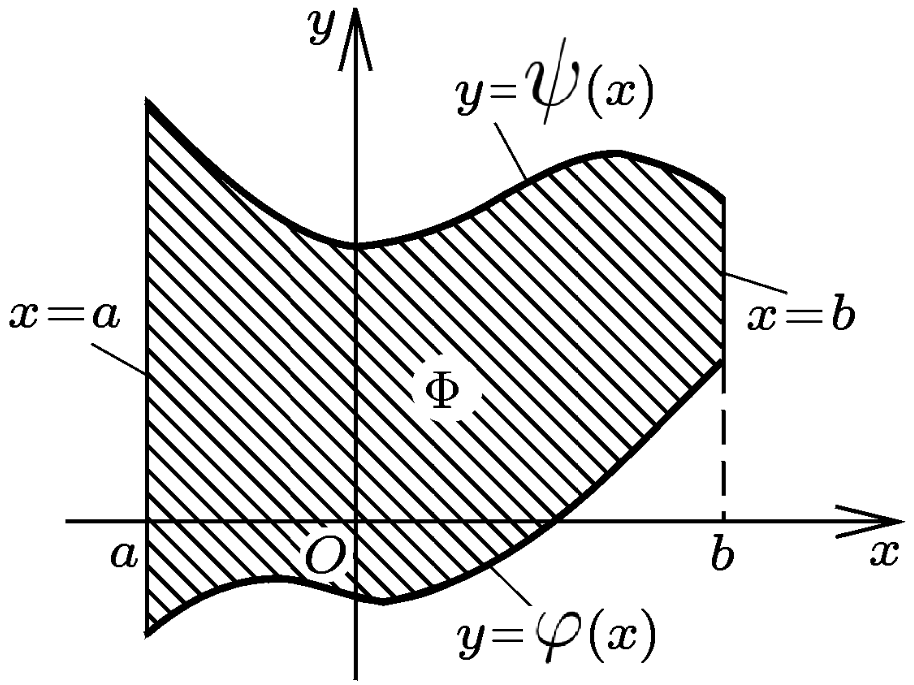
\includegraphics[width=\textwidth]{images/scren_16.png}
Область элементарная отн. Oy
\end{minipage}

\begin{definition}
    Область в $\R^2$ называется \textit{элементарной}, если она элементарна относительно одной из осей.
\end{definition}

\hypertarget{lemma_8_6}{}
\begin{lemma}[о разбиении б/д]
    Пусть $G \subset \R^2$~---~область, граница которой состоит из конечного числа дизъюнктивных простых кусочно-гладких контуров $\{\Gamma_i\}_{i = 1}^N$. Тогда она может быть <<правильно>> \  разбита на конечное число элементарных областей, т.е. $\exists \{G_j\}_1^M$:
    \begin{enumerate}
        \item $G_i \cap G_j = \emptyset$
        \item $G_i \subset G$
        \item $\bigcup \overline{G_i} = \overline{G}$
        \item $\partial G_i \cap \partial G_j \cap G$ либо пусто, либо состоит из одной точки, либо является промежутком.
    \end{enumerate}
\end{lemma}
\begin{note}
    Нижеприведённый текст не является официальным доказательством, сформулирован достаточно неформально и по сути своей является лишь идеей доказательства (быть может не полностью корректной).
\end{note}
\begin{proof}
    Заметим, что нам достаточно покрыть границу $G$ конечным числом прямоугольников (стороны которых параллельны координатным осям) так, что пересечение внутренности каждого из них с $G$ было элементарным, поскольку после вычитания из $G$ всех таких прямоугольников у нас останется область, границы которой параллельны координатным осям -- такую область можно без каких-либо проблем разбить на объединение прямоугольников требуемым образом. \\
    Ввиду открытости области мы можем выбирать настолько малые прямоугольники, чтобы в принципе не обращать внимание на другие простые кусочно-гладкие контуры при организации разбиения $\Gamma_i$. \\
    У каждого из простых кусочно-гладких контуров есть конечное число особых точек (в данном контексте - точек, где $r'(t)$ не является непрерывной) и конечное число точек перехода через ноль у $r'(t)$ (то есть таких точек $t_0$, что или $x'(t_0) = 0$, или $y'(t_0) = 0$, причём или при $t_0 - 0$, или при $t_0 + 0$ они не равны нулю). Накроем их достаточно малыми прямоугольниками, так, чтобы в один прямоугольник попала только одна такая точка. Теперь, очевидно, что оставшиеся гладкие отрезки кривых можно хорошо покрыть прямоугольниками -- они монотонны относительно одной из осей. Всякую точку перехода через 0, не являющуюся особой тоже можно покрыть без проблем: просто одна из функций $\phi/\psi$ не будет монотонной. Для хорошего покрытия особой точки, нам, быть может, потребуется разрезать получившийся прямоугольник на две части.
\end{proof}






\begin{theorem}[Формула Грина]
    Пусть $G \subset \R^2$~---~область: $\partial G$ состоит из дизъюнктивного объединения простых кусочно-гладких контуров $\{\Gamma_i\}_{i = 1}^N$. Пусть $\forall i \in \overline{1, \ldots, N}$ $\Gamma_i^+$ положительно  ориентирована относительно $G$, $\displaystyle \partial G^+ := \bigsqcup_{i = 1}^{N} \Gamma_i^+$. Пусть $F \in C^1(\overline{G}, \R^2)$. Тогда, если $F = (P \  Q)^T$, то \[\int\limits_{\partial G^+} (F, dr) = \int\limits_{\partial G^+} Pdx + Qdy = \iint\limits_G \left(\dfrac{\partial Q}{\partial x} - \dfrac{\partial P}{\partial y}\right) dxdy\]
\end{theorem}
\begin{proof}
    $F = F_1 + F_2, F_1 = (P \  0)^T, F_2 = (0 \  Q)^T$. Теорему достаточно доказать для $F_1$, доказательство для $F_2$ аналогично. Будем последовательно усложнять область $G$(на картинках показана эволюция нашей области):\\

\noindent 
\begin{minipage}{0.3\textwidth}
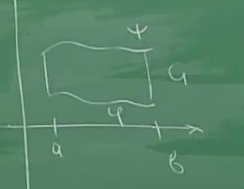
\includegraphics[width=\textwidth]{images/Grin_step1.png}
Шаг 1.
\end{minipage}
\begin{minipage}{0.3\textwidth}
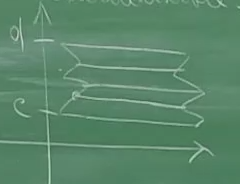
\includegraphics[width=\textwidth]{images/Grin_step2.png}
Шаг 2.
\end{minipage}
\begin{minipage}{0.365\textwidth}
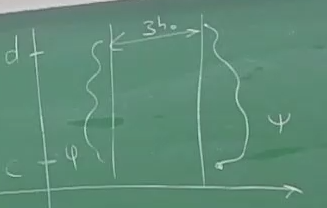
\includegraphics[width=\textwidth]{images/Grin_step3.png}
Шаг 3.
\end{minipage}
\vspace{10pt}

\textbf{\underline{Шаг 1.}} Будем считать $G$ элементарной относительно $Oy$: \[G = \{(x, y) \mid x \in (a, b), y \in (\phi(x), \psi(x))\}\] Тогда по теореме Фубини и учитывая что $\dfrac{\partial P}{\partial y}$ непрерывно дифференцируема, а значит интеграл Лебега совпадает с интегралом Риммана и по формуле Ньютона-Лейбнциа:\[\iint\limits_G \dfrac{\partial P}{\partial y}dxdy = \int\limits_{a}^b dx\int\limits_{\phi(x)}^{\psi(x)} \dfrac{\partial P}{\partial y} dy = \int\limits_a^b \Big( P(x, \psi(x)) - P(x, \phi(x)) \Big) dx\]
Полагая $\Gamma_1 = \{r = (x, \phi(x)) \mid x \in [a, b]\}$ и $\Gamma_2 = \{\rho = (x, \psi(x)) \mid x \in [a, b]\}$, можем заметить, что $r'(x) = (1, \phi'(x))$ и $\rho'(x) = (1, \psi'(x))$. Но, Тогда \[\int\limits_a^b P(x, \phi(x))dx = \int\limits_{\Gamma_1^+} (F_1, dr)\]
    \[-\int\limits_a^b P(x, \psi(x))dx = \int\limits_{\Gamma_2^+} (F_1, dr)\]
    Поскольку вторая компонента поля $F_1$ нулевая, то интеграл по вертикальным отрезкам нулевой, а значит в этом случае формула доказана.\\
    \textbf{\underline{Шаг 2.}} Пусть область $G$ элементарна относительно $Ox$: \[G = \{(x, y) \mid y \in (c, d), x \in (\phi(y), \psi(y))\}\]
        Предположим, дополнительно, что $\phi$ и $\psi$~---~кусочно-линейные. Если брать картинку, то края уже не отрезки, а ломаные, т.е. $\exists T = \{t_i\}_{t = 0}^{N}$ т.ч. $c = t_0 < t_1 < \ldots < t_N = d$ и $\phi|_{[t_i, t_{i + 1}]}, \psi|_{[t_i, t_{i + 1}]}$~---~отрезки. Тогда на каждой из областей $G_i$, на которые $G$ делится прямыми $y = t_i$, справедливость формулы Грина уже показана: \[\iint_{G_i} \dfrac{\partial P}{\partial y}dxdy = - \int\limits_{\partial G_i^+} Pdx\]
        Теперь, заметим, что формула Грина верна и для объединения всех этих областей, поскольку $\iint$ аддитивен по множествам $G_i$, а объединением кривых $\partial G_i^+$ будет $\partial G^+$, поскольку на прямой $y = t_{i + 1}$ где пересекаются $\partial G_i^+$ и $\partial G_{i + 1}^+$ интегралы по отрезку "выпиливаются" друг об друга, поскольку имеют противоположные направления. \\
    \textbf{\underline{Шаг 3.}} Пусть область $G$~---~элементарна относительно $Ox$, а $\phi$ и $\psi$~---~произвольные непрерывные и кусочно непрерывно-дифференцируемые на $[c, d]$: \[G = \{(x, y) \mid y \in (c, d), x \in (\phi(y), \psi(y))\}\]
        И, при этом, $\exists h_0 > 0$ т.ч. $\forall y \in [c, d] \hookrightarrow \psi(y) - \phi(y) \geq 3h_0$, чтобы зазор между кривыми не "схлопнулся". Зафиксируем $h \in (0, h_0)$. Сдвинем $\phi$ на $h$ вправо, а $\psi$~---~на $h$ влево, и получим некоторые кривые $\Gamma_{1, h} = \Gamma_1 + (h, 0)$ и $\Gamma_{2, h} = \Gamma_2 - (h, 0)$ и функции $\psi_h = \psi - h, \phi_h = \phi + h$.\\
        Пусть $T = \{t_i\}$~---~разбиение отрезка $[c, d]$ с достаточно малой мелкостью, а $\phi_h^T$ и $\psi_h^T$~---~порождённые этим разбиением ломаные не пересекаются т.ч. $\phi(y) < \phi_h^T(y) < \phi(y) + 3/2h$ и $\psi(y) - 3/2h < \psi_h^T(y) < \psi(y)$. Такая мелкость существует, поскольку $\psi$ и $\phi$~---~кусочно 1-гладкие и $\exists \max |\psi'(y)|$ и $\exists \max |\phi'(y)|$. Пусть $G_h$~---~область, запертая между $\phi_h$ и $\psi_h$, а $G_{h}^T$~---~область, запертая между $\phi_h^T$ и $\psi_h^T$. По предыдущему шагу мы имеем \[\iint\limits_{G_h^T} \dfrac{\partial P}{\partial y}dxdy = -\int\limits_{(\partial G_h^T)^+} Pdx\]
        \hyperlink{krivaya_lomanaya}{По лемме о приближении кривой ломанными}\[\int\limits_{(\Gamma_{i, h}^T)^+} Pdx \longrightarrow \int\limits_{(\Gamma_{i, h})^+}Pdx, \  l(T) \rightarrow 0\]
         С другой стороны, \[\biggr|\iint\limits_{G_h^T}\dfrac{\partial P}{\partial y} dxdy - \iint\limits_{G_h}\dfrac{\partial P}{\partial y}dxdy\biggr| \leq \max\limits_{\overline{G}}|\dfrac{\partial P}{\partial y}|\cdot |\LL^2(G_h^T \triangle G_h)| \rightarrow 0, \  l(T) \rightarrow 0\]
        Таким образом формулу Грина верна для $G_h$. \\
        Устремим $h \rightarrow +0$, используя теорему Фубини:
        \[\biggr|\iint\limits_G \dfrac{\partial P}{\partial y} dxdy - \iint\limits_{G_h} \dfrac{\partial P}{\partial y} dxdy\biggr| \leq \max\limits_{\overline{G}} |\dfrac{\partial P}{\partial y}| \LL^2(G \triangle G_h) \leq M \cdot 2h \cdot |c -d| \rightarrow 0, h \rightarrow +0\]
        Теперь покажем, что $\int\limits_{\partial G_h^+} Pdx \rightarrow \int\limits_{\partial G^+} Pdx, h \rightarrow +0$.
        Для этого достаточно показать, что $\int\limits_{\Gamma_{i, h}}Pdx \rightarrow \int\limits_{\Gamma_i} Pdx, h \rightarrow +0$.
        Тогда \[\biggr|\int\limits_{\Gamma_{1, h}}Pdx - \int\limits_{\Gamma_1}Pdx\biggr| = \int\limits_{c}^{d} |P(\phi(y) + h, y) - P(\phi(y), y)|\cdot|\phi'(y)|dy \leq \]\[ \leq |c - d|\max\limits_{[c, d]}|\phi'(y)| \max\limits_{[c, d]}|P(\phi(y), y) - P(\phi(y) + h, y)| \rightarrow 0, h \rightarrow 0\]
        Таким образом этот шаг доказан.\\
    \textbf{\underline{Шаг 4.}} Предположим теперь что $G$~---~проста относительно $Ox$. Теперь не запрещается чтобы $\phi(d) = \psi(d), \psi(c) = \phi(c)$; напомним, что $\phi < \psi$ на $(c, d)$ и $\phi, \psi$~---~непрерывные и кусочно непрерывно-дифференцируемые. Зафиксируем некоторое $\epsilon > 0$. Рассмотри $G_\epsilon = \{(x, y) \mid c + \epsilon < y < d - \epsilon, x \in (\phi(y), \psi(y))\}$. Так как $\psi \phi \in C([c, d])$ и $\phi - \phi > 0$ на отрезке $[c + \epsilon; d - \epsilon ]$, непрерывная функция на отрезке достигает минимума и она положительна, а значит $\exists h_0 > 0: \psi - \phi \geq 3h_0 \forall y \in [c + \epsilon; d - \epsilon ]$ Для $G_\epsilon$ утверждение доказано на предыдущем шаге. Тогда \[\iint\limits_G \dfrac{\partial P}{\partial y} dxdy = \iint\limits_{G_\epsilon} P'_ydxdy = -\int\limits_{\partial G_\epsilon^+} Pdx\]
    Устремим $\epsilon$ к 0: \[\biggr|\iint\limits_G P'_ydxdy - \iint\limits_{G_\epsilon} P'_ydxdy\biggr| = \biggr|\iint\limits_{G \setminus G_\epsilon}P'_ydxdy\biggr| \leq \max\limits_{\overline{G}}\biggr|\dfrac{\partial P}{\partial y}\biggr||\LL^2(G \setminus G_\epsilon)| \rightarrow 0, \epsilon \rightarrow 0\]
    Пусть $\Gamma_3$ и $\Gamma_4$~---~это $G|_{y = c}$ и $G|_{y = d}$ соответственно, а $\Gamma_{3, \epsilon} = G_\epsilon|_{y = c + \epsilon}$ и $\Gamma_{4, \epsilon} = G_\epsilon|_{y = d - \epsilon}$. Очевидно, что к <<боковым>> кривым $\Gamma_1 = \{(\psi(y), y) \mid y \in (c, d)\}$ и $\Gamma_2 = \{(\phi(y), y) \mid y \in (c, d)\}$ сходятся $\Gamma_{1, \epsilon} = \{(\psi(y), y) \mid y \in (c + \epsilon, d - \epsilon)\}$ и $\Gamma_{2, \epsilon} = \{(\phi(y), y) \mid y \in (c + \epsilon, d - \epsilon)\}$ и соответственно сходятся интегралы по этим кривым. Если $\Gamma_3$~---~точка, то очевидно, что $\int\limits_{\Gamma_{3, \epsilon}} Pdx \rightarrow \int\limits_{\Gamma_{3}} Pdx, \epsilon \rightarrow 0$. Иначе \[\biggr|\int\limits_{\Gamma_{3, \epsilon}}P(x, c + \epsilon)dx - \int\limits_{\Gamma_3}P(x, c)dx\biggr| \leq \]\[ \leq \int\limits_{\alpha(x)}^{\beta(x)} |P(x, c + \epsilon) - P(x)|dx + \int\limits_{\Delta_1(\epsilon) \cup \Delta_2(\epsilon)} \max(|P(x, c + \epsilon)|, |P(x, c)|)dx \rightarrow 0, \epsilon \rightarrow 0.\]
    \textbf{\underline{Шаг 5.}} \hyperlink{lemma_8_6}{Применяя лемму о разбиении} мы получаем конечное множество элементарных областей, удовлетворяющих условиям леммы $\{G_i\}_{i = 1}^N$. Для каждого $G_i$ мы можем применить уже доказанное и получить: \[\iint\limits_{G_i} Q'_x - P'_ydxdy = \int\limits_{G_i^+} Pdx+Qdy.\]
    Очевидно, что \[\sum\limits_{i = 1}^N \iint\limits_{G_i} Q'_x - P'_ydxdy = \iint\limits_G Q'_x - P'_ydxdy.\]
    Для каждого $i \in 1, \{\ldots, N\}$ определим внутреннюю границу $\partial^iG_i^+ = \partial G_i^+ \cap G$ и внешнюю границу $\partial^e G_i^+ = \partial G_i^+ \cap \partial G$. Ясно, что \[\bigcup\limits_{i = 1}^N \partial^e G_i^+ = \partial G^+.\]
    Тогда \[\sum\limits_{i = 1}^N \int\limits_{\partial^e G_i^+} Pdx + Qdy = \int\limits_{\partial G^+} Pdx + Qdy.\]
    Пусть $\partial^i G_i^+ \neq \emptyset$. Пусть существует такое $j$, что $\partial^iG_i^+ \cap \partial^i G_j^+ \neq \emptyset$ и пусть они пересекаются по промежутку (случай пересечения по точке тривиален). Тогда пересечение -- это промежуток, наделённый двумя противоположными ориентациями. Но тогда \[\sum\limits_{i = 1}^N \int\limits_{\partial^i G_i^+} Pdx + Qdy = 0.\]
    Из этого следует необходимое равенство и получается утверждение теоремы.

\end{proof}